% Author: Alfredo Sánchez Alberca (asalber@ceu.es)
% !TEX program: pdflatex
\documentclass[fleqn,10pt]{wlscirep}
\usepackage[utf8]{inputenc}
\usepackage[T1]{fontenc}
\usepackage{array}
\usepackage{caption}
\usepackage{subcaption}
\usepackage{booktabs}

\title{Clinical-evolutionary staging system of primary open-angle glaucoma using optical coherence tomography}

\author[1,*]{Alfonso Parra-Blesa}
\author[1]{Alfredo Sánchez-Alberca}
\author[2]{José J. García-Medina}
\affil[1]{San Pablo CEU, , Madrid, Spain}
\affil[2]{Malaga, Spain}

\affil[*]{alf.parra.ce@ceindo.ceu.es}

%\keywords{Keyword1, Keyword2, Keyword3}

\begin{abstract}
We propose a new and objective algorithm for classifying primary open-angle glaucoma (POAG) into clinical-evolutionary stages using spectral domain optical coherence tomography (SD-OCT). We enrolled 1001 patients in this study, 235 of whom were glaucomatous and at different stages of the disease. The Heidelberg Spectralis SD-OCT device (version 6.7) was used, which allowed us to determine the thicknesses of rims 3.0, 4.1, and 4.7 of the peripapillary retinal nerve fibre layer (RNFL) and Bruch's membrane opening-minimum rim width (BMO-MRW). All rims were divided into seven variables (G-T-TS-TI-N-NS-NI), which were normalized according to the formula provided by Heidelberg Engineering, GmbH, Germany, with correction for age and papillary distortion factors. The k-means algorithm and linear discriminant analysis were used to classify patients into four disease stages.  We defined four glaucoma stages and provided a new model for classifying eyes in these stages, with an overall accuracy greater than 92\% (88\% when including healthy eyes). An online application was also implemented to predict the probability of glaucoma stage for any given eye. This classification system can easily be applied to large populations for glaucoma screening and provides a common and objective language among ophthalmologists.
\end{abstract}
\begin{document}

\flushbottom
\maketitle

\thispagestyle{empty}

%\noindent Please note: Abbreviations should be introduced at the first mention in the main text – no abbreviations lists. Suggested structure of main text (not enforced) is provided below.

\section*{Introduction}

The function of a correct classification system is to highlight the essential and defining elements in a group of related phenomena to facilitate practical decision making. The main difficulty encountered in medical science is identifying a criterion that can frame all forms of a disease such as glaucoma in a coherent system to offer direct therapeutic suggestions \cite{society:2017:terminology}. The objective of this study is to identify an essential element that allows us to develop a clinical-evolutionary classification system for primary open-angle glaucoma (POAG).

Glaucoma is considered one of the main causes of blindness, and based on this relationship, the WHO specifically recommends early diagnosis and treatment for blindness prevention \cite{thylefors:1994:bull}.

Many aetiopathogenic classifications of glaucoma have been proposed in recent years, including the system presented by Ourgaud, Etienne, and Krasnov at the European Glaucoma Society in 2008, which was ratified in 2017 \cite{society:2017:terminology, krasnov:1965:pathogenic, etiennerourgaud:1961:lexploration}.

The emergence of optical coherence tomography (OCT) in 1991 based on the work of D. Huang and Fujimoto \cite{huang:1991:optical} affected not only the aetiopathogenic classification but also the understanding and management of POAG and its pathophysiology, which has allowed us to diagnose the disease earlier.

The visual field (VF) has provided information about the evolution of glaucoma and its diagnosis, but its subjective nature and late significance with respect to the onset of the disease, which requires a loss of 40\% of the retinal ganglion cells, limits its use as an element for early diagnosis\cite{quigley:1982:optic}.

The non-invasive nature of OCT coupled with its ability to quantify the macular layers of the retina and the peripapillary retinal nerve fibre layer (RNFL), its reproducibility, and its ability to provide standardized data on the evolution of Bruch's membrane opening-minimum rim width (BMO-MRW)\cite{schuman:1995:quantification} helps us better monitor and diagnose glaucoma early\cite{bengtssonb:2012:performance, grewal:2013:diagnostico, lee:2010:reproducibility, toteberg-harms:2012:repeatability}. \textbf{Huang, L., 2011 (esta referencia no está en la bibliografía)}. 

Spectral domain optical coherence tomography (SD-OCT) provides objective values reflecting damage to the BMO-MRW and RNFL, not only improving knowledge about these structures but also allowing the development of an objective, reproducible, and accessible clinical-evolutionary classification system with greater sensitivity than the VF, thus yielding a common language for the evolution of the disease\cite{balwuantray:2013:, zhang:2017:comparison}.

This work aims to define a new clinical-evolutionary classification of POAG based on the k-means algorithm using objective BMO-MRW data acquired from SD-OCT.

\section*{Results}

\subsection*{The sample and variables}

For the study sample, 1001 individuals were selected (235 with glaucoma and 766 without glaucoma). To avoid a natural correlation between the eyes of the same individuals, only left eyes were considered.

For each eye, the main variables measured through OCT were the thickness of the BMO-MRW at the temporal inferior (BMO-MRW.TI), temporal (BMO-MRW.T), temporal superior (BMO-MRW.TS), nasal superior (BMO-MRW.NS), nasal (BMO-MRW.N), nasal inferior (BMO-MRW.NI) and general (BMO-MRW.G) sectors, the thickness of the 3.5 rim of the RNFL at the temporal inferior (Rim3.5.TI), temporal (Rim3.5.T), temporal superior (Rim3.5.TS), nasal superior (Rim3.5.NS), nasal (Rim3.5.N), nasal inferior (Rim3.5.NI) and general (Rim3.5.G) sectors,  the thickness of the 4.1 rim of the RNFL at the temporal inferior (Rim4.1.TI), temporal (Rim4.1.T), temporal superior (Rim4.1.TS), nasal superior (Rim4.1.NS), nasal (Rim4.1.N), nasal inferior (Rim4.1.NI) and general (Rim4.1.G) sectors, and the thickness of the 4.7 rim of the RNFL at the temporal inferior (Rim4.7.TI), temporal (Rim4.7.T), temporal superior (Rim4.7.TS), nasal superior (Rim4.7.NS), nasal (Rim4.7.N), nasal inferior (Rim4.7.NI) and general (Rim4.7.G) sectors. The individuals’ ages and BMO-MRW areas were also documented for standardization.

\subsection*{Correlation analysis}

Correlation analysis (Figure~\ref{fig:correlation}) showed a clear correlation pattern by sectors. A very strong Pearson correlation ($r > 0.9$) was identified among the thickness of the BMO-MRW and RNFL rims 3.5, 4.1 and 4.7 by sectors. A strong correlation ($r > 0.75$) was also found among the sectors of the BMO-MRW, except for the BMO-MRW.G, which presented a very strong correlation with the other sectors. On the other hand, a very weak correlation ($r < 0.2$) was found between the T sector and the N, NI and NS sectors.

\begin{figure}[ht]
\centering
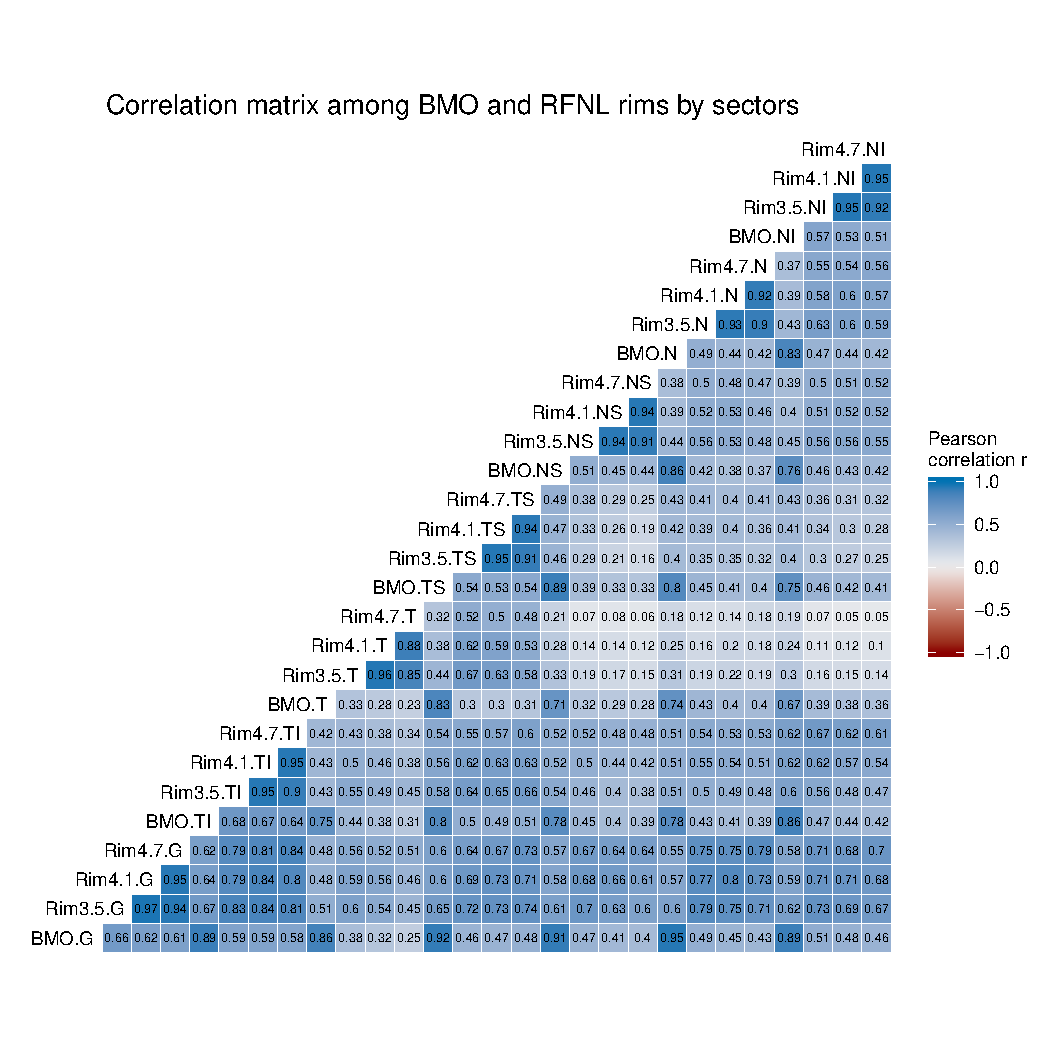
\includegraphics[width=0.5\linewidth]{img/correlation-matrix-bmo-rnfl.pdf}
\caption{Correlation matrix map among the thickness of the BMO-MRW and RNFL rims by sectors. Every cell represents the Pearson correlation coefficient r of the variables at the corresponding row and column. Light blue represents a strong correlation, and dark blue represents a weak correlation.}
\label{fig:correlation}
\end{figure}

\subsection*{Principal component analysis}

Since most of the variables were highly correlated, principal component analysis was performed to reduce the dimensionality of the data and determine which variables explained most of the variability of the data. Principal component analysis is a statistical method used to reduce the dimensionality of data by transforming the original variables (usually correlated) into a new set of linearly uncorrelated variables. The first principal component is a linear combination of variables that explain the highest variability in the data (the maximum variance), and the second principal component is a linear combination of variables with the maximum variance, which is orthogonal to the first component\cite{hassel:2009:}.

Figure~\ref{fig:variability-explained-pca} shows that the first principal component explains almost 60\% of the total variability of the data, while the second and third principal components explain only 11\% and 9\% of the total variability.

\begin{figure}[ht]
\centering
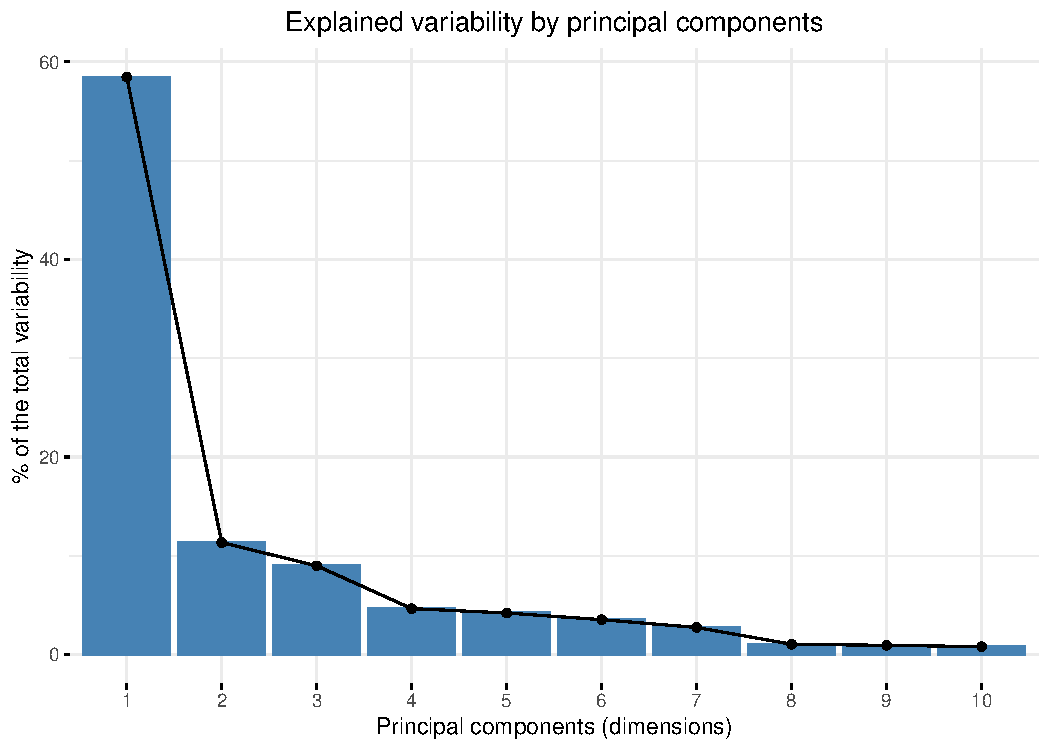
\includegraphics[width=0.5\linewidth]{img/explained-variability-principal-components.pdf}
\caption{Percentage of the total variability explained by the main principal components.}
\label{fig:variability-explained-pca}
\end{figure}

Plotting the subjects’ eyes on the first two principal components (Figure~\ref{fig:pca-map}) reveals that healthy eyes can easily be discriminated from glaucoma eyes along the first principal component (horizontal dimension), with a small overlapping area, which is not possible at all along the second principal component (vertical dimension).

\begin{figure}[ht]
\centering
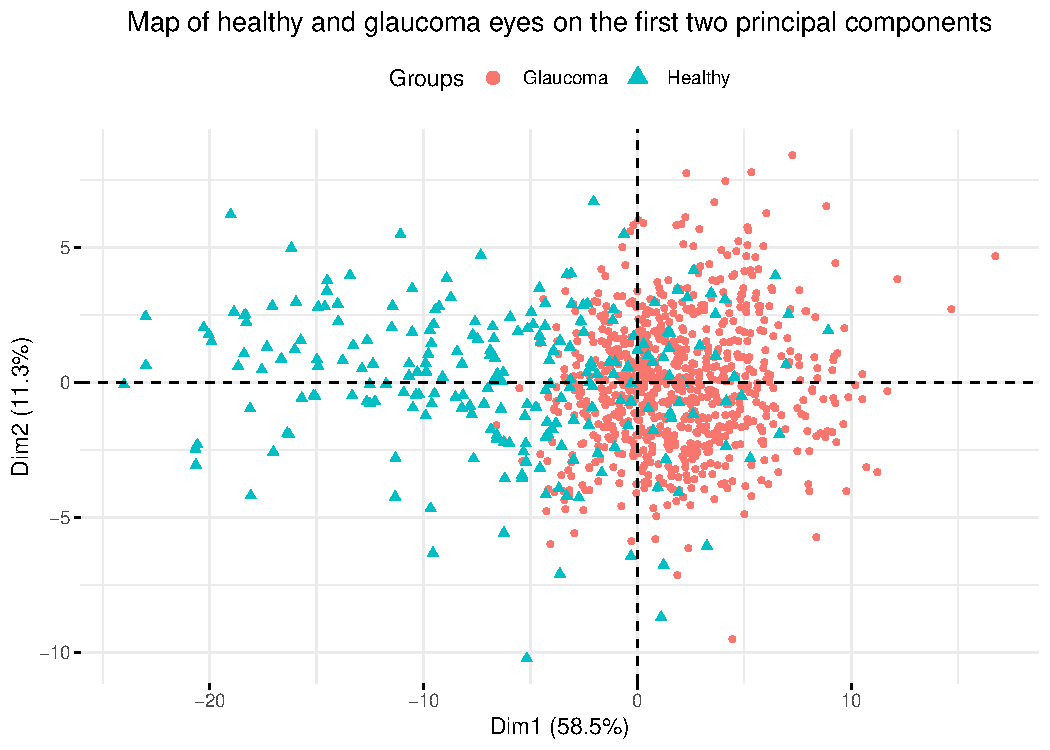
\includegraphics[width=0.5\linewidth]{img/pca-map.pdf}
\caption{Map of healthy and glaucoma eyes on the first two principal components. The horizontal dimension (x-axis) corresponds to the first principal component, and the vertical dimension (y-axis) corresponds to the second principal component.}
\label{fig:pca-map}
\end{figure}

On the other hand, according to Figure~\ref{fig:correlation-pca}, the variables that are more correlated with the first principal component are sectors G and TI of all the rims.

\begin{figure}[ht]
\centering
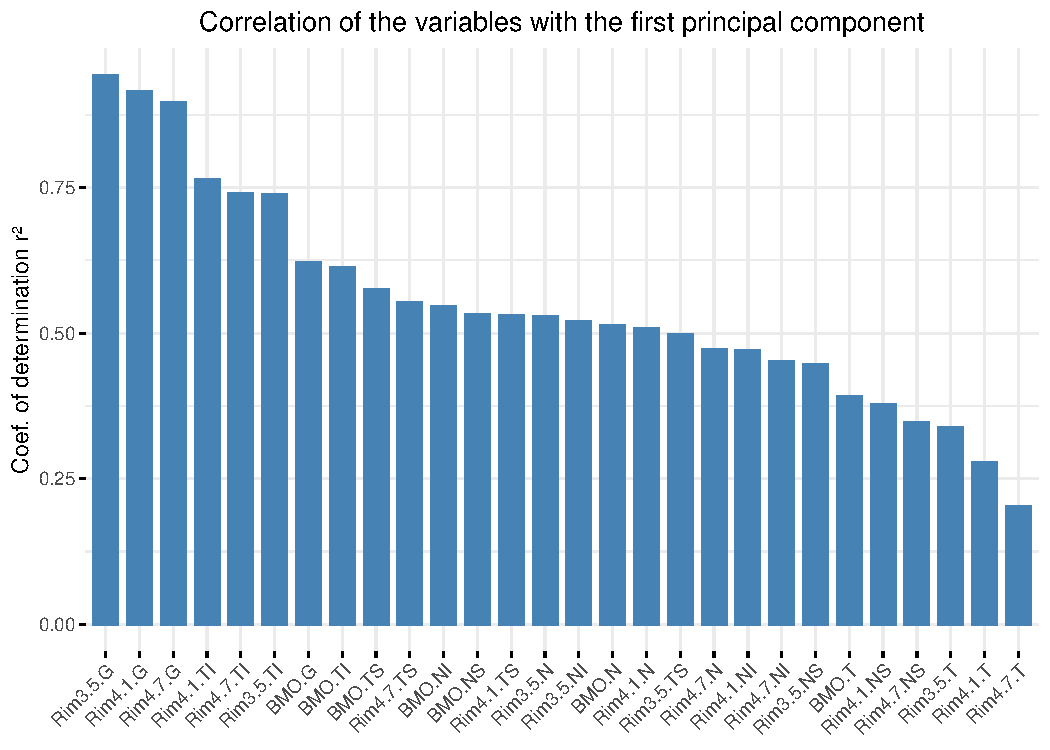
\includegraphics[width=0.5\linewidth]{img/correlation-pca.pdf}
\caption{Correlations of the BMO-MRW and RNFL rim variables with the first principal component.}
\label{fig:correlation-pca}
\end{figure}

\subsection*{Cluster analysis}

To define the severity stages of glaucoma, we applied the k-means cluster algorithm to the BMO-MRW and RNFL variables of eyes with glaucoma. This algorithm groups eyes into k clusters or classes according to the Euclidean distance from the eye to the cluster centroids in the n-dimensional space of the variables. Every eye is assigned to the cluster with the closest centroid (1). Based on Figure~\ref{fig:reduction-variability-clusters}, which shows the reduction in intra-group variability when we increase the number of clusters, we decided to create four clusters since reducing intra-group variability is not important for more than four groups (elbow criteria)\cite{kassambara:2017:practical}. We have named these clusters I, II, III, and IV in the order of increasing severity.

\begin{figure}[ht]
\centering
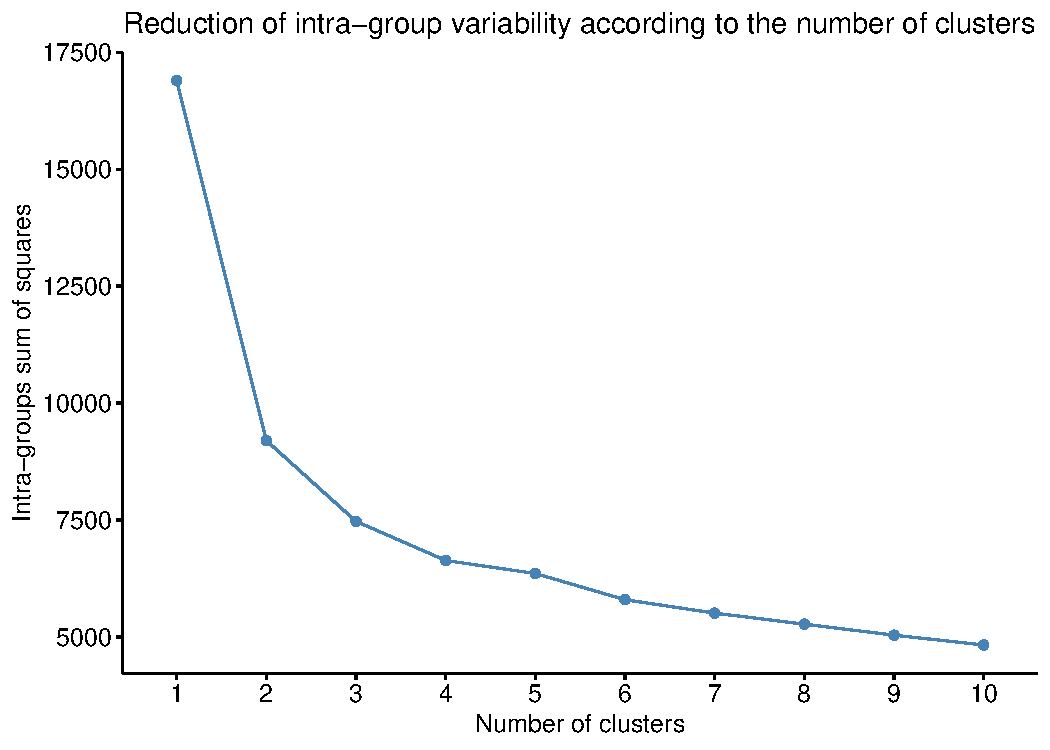
\includegraphics[width=0.5\linewidth]{img/reduction-variability-clusters.pdf}
\caption{Reduction in the intra-group variability with an increasing number of clusters. According to the elbow criteria, the optimal number of clusters is 3 or 4.}
\label{fig:reduction-variability-clusters}
\end{figure}

Figure~\ref{fig:clusters-whithout-healty-eyes} shows the clusters on the axes corresponding to the first two principal components. As shown in this chart, the four clusters can be separated almost perfectly along the x-axis of the first principal component.

\begin{figure}
\centering
\begin{subfigure}[b]{0.49\textwidth}
\centering
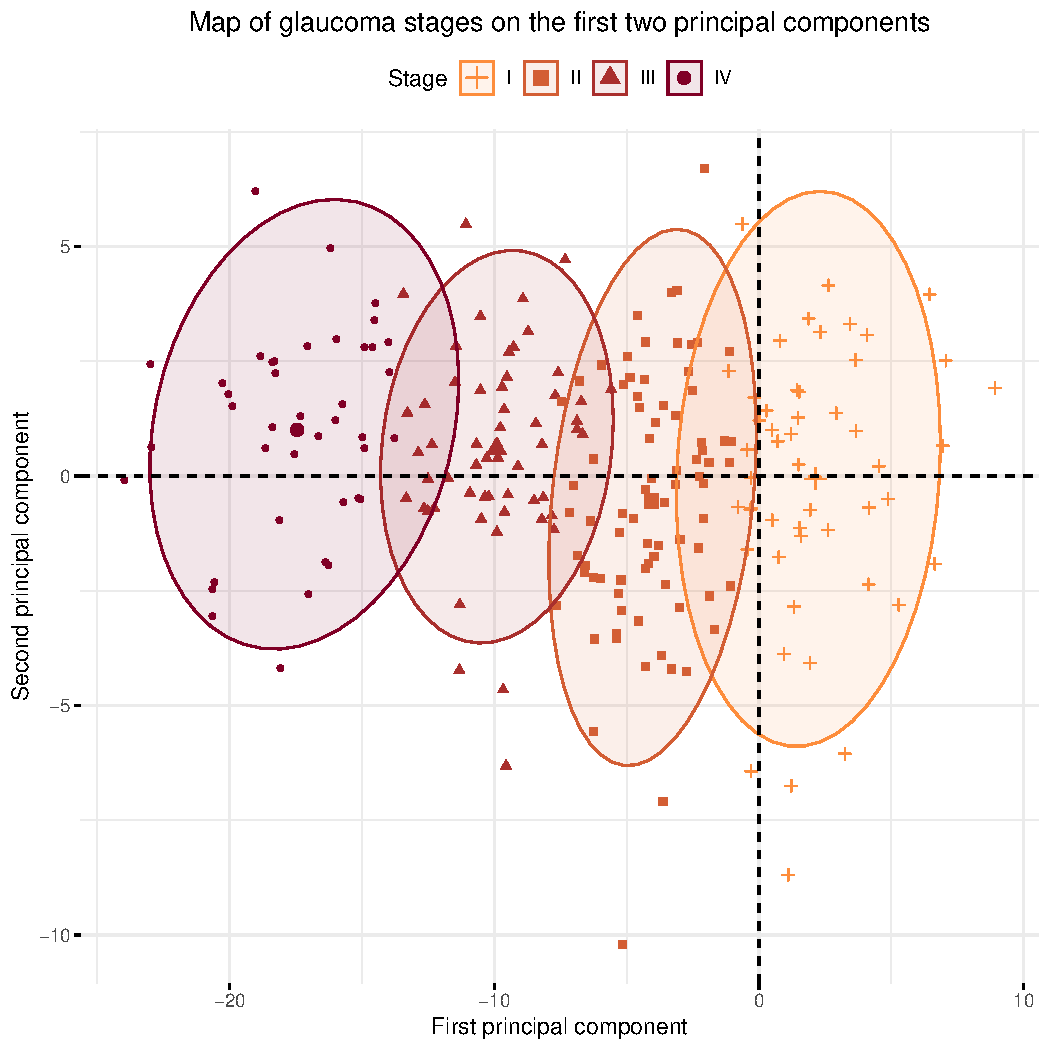
\includegraphics[width=\textwidth]{img/map-clusters-whithout-healthy.pdf}
\caption{Clusters without healthy eyes.}
\label{fig:clusters-whithout-healty-eyes}
\end{subfigure}
%\hfill
\begin{subfigure}[b]{0.49\textwidth}
\centering
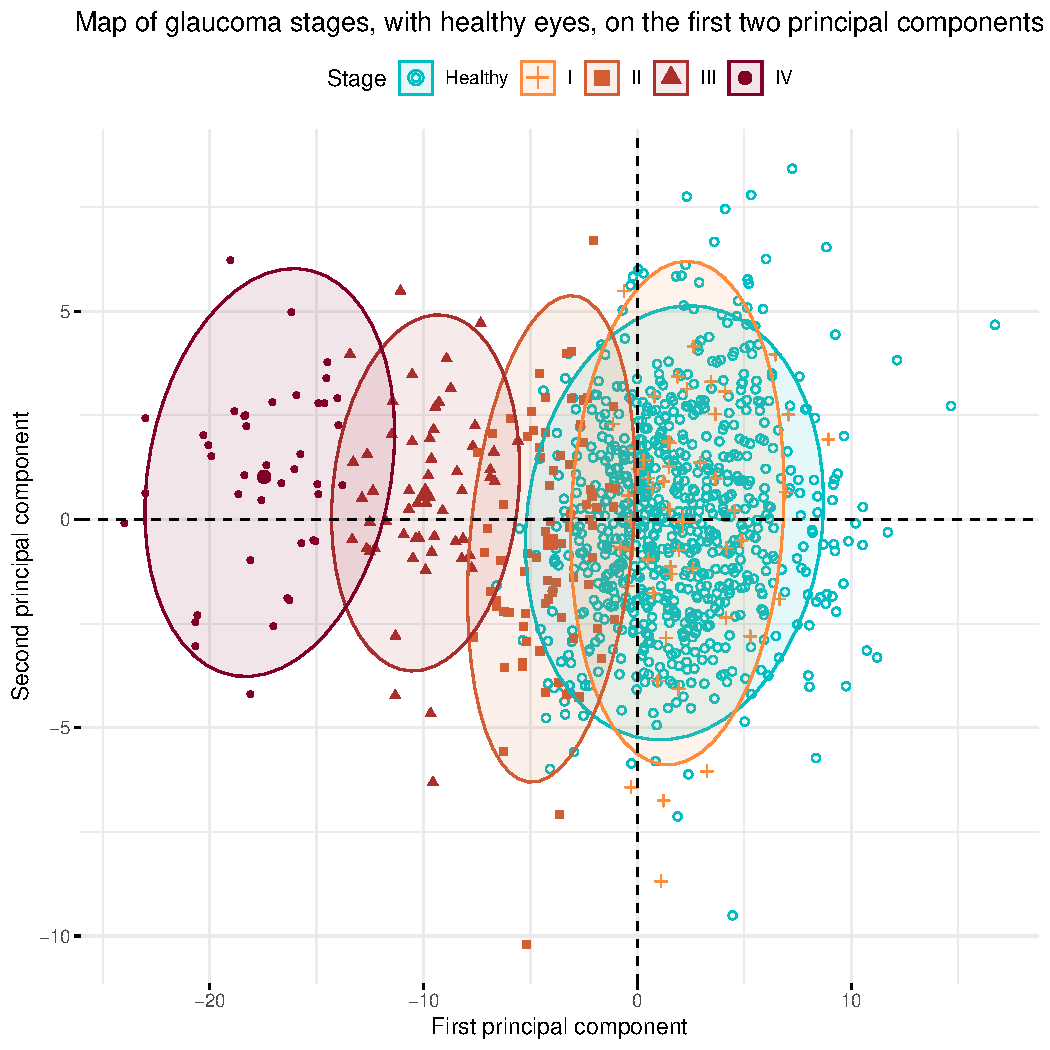
\includegraphics[width=\textwidth]{img/map-clusters-with-healthy.pdf}
\caption{Clusters with healthy eyes.}
\label{fig:clusters-with-healthy-eyes}
\end{subfigure}
\caption{Clusters defined by the k-means method using all the BMO-MRW and RNFL rim variables represented on the x-axis and y-axis corresponding to the first and second principal components, respectively.}
\label{fig:clusters}
\end{figure}

To determine whether the classes detected were related to the severity of glaucoma, that is, whether a gradient of severity existed from cluster I to cluster IV, we added healthy eyes to the previous plot. In Figure~\ref{fig:clusters-with-healthy-eyes}, we can see that healthy eyes were plotted to the right of the x-axis (corresponding to the first principal component), overlapping with the eyes of cluster I and partially overlapping with the eyes of cluster II. This finding is logical since cluster I contains eyes in the early stages of glaucoma, which are not very different from healthy eyes. Clusters III and IV are located at the other end of the x-axis far from the healthy eyes, which correspond to eyes with more severe glaucoma. We can see that these clusters do not overlap with healthy eyes, which is even clearer in Figure~\ref{fig:clusters-distributions} showing the distribution of the first principal component for every glaucoma stage and healthy eyes.

\begin{figure}[ht]
\centering
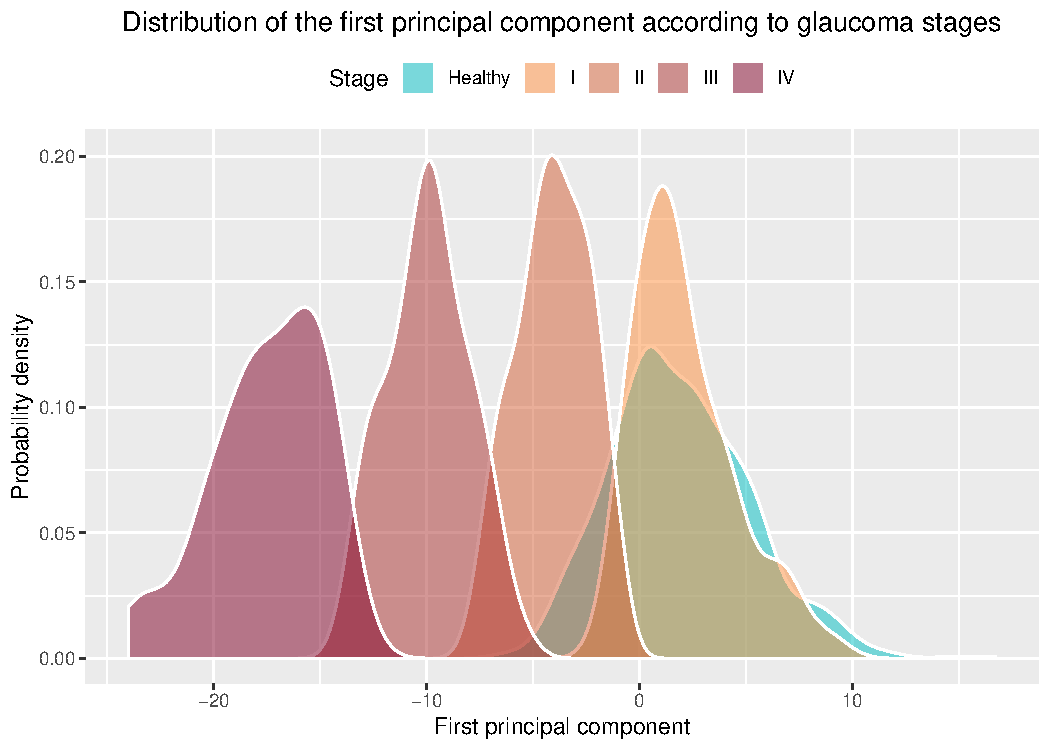
\includegraphics[width=0.5\linewidth]{img/clusters-distributions.pdf}
\caption{Distribution of the first principal component of the BMO-MRW and RNFL rim variables by glaucoma stages and healthy eyes.}
\label{fig:clusters-distributions}
\end{figure}

\subsection*{Linear discriminant analysis}

After defining the clusters, we applied linear discriminant analysis (LDA) to determine whether the four defined stages can be easily predicted. LDA is a statistical method used to identify a set of discriminant functions, all of which are uncorrelated linear combinations of the variables, that maximizes the difference between classes and separates the classes the best\cite{hassel:2009:}. The number of discriminant functions created is the number of classes minus one, which is three in our study.

LDA was applied to the principal components of the BMO-MRW and RNFL rim variables since the original variables were highly correlated. Previously, we assessed the normality and homogeneity of variances of the principal components.

As shown in Table~\ref{tab:classification1-whithout-healthy}, the four classes of glaucoma could be predicted with very high sensitivity ($> 0.9$) and specificity ($> 0.95$), and $92.9\%$ of the eyes were classified correctly. 

\begin{table}[h]
\begin{subtable}[b]{0.5\textwidth}
\centering
\begin{tabular}{lrr>{\raggedleft\arraybackslash}m{1.5cm}}
\toprule
& \bf Sensitivity & \bf Specificity & \bf Balanced\newline accuracy \\
Stage I & 0.92 & 0.99 & 0.96 \\ 
Stage II & 0.97 & 0.95 & 0.96 \\ 
Stage III & 0.89 & 0.98 & 0.93 \\ 
Stage IV & 0.90 & 0.98 & 0.94 \\ 
\bottomrule
\end{tabular}
\caption{Classification without healthy eyes.}
\label{tab:classification1-whithout-healthy}
\end{subtable}
\hfill
\begin{subtable}[b]{0.5\textwidth}
\centering
\begin{tabular}{lrr>{\raggedleft\arraybackslash}m{1.5cm}}
\toprule
& \bf Sensitivity & \bf Specificity & \bf Balanced\newline accuracy \\
Stage Healthy & 0.98 & 0.65 & 0.82 \\ 
Stage I & 0.18 & 0.99 & 0.58 \\ 
Stage II & 0.46 & 0.98 & 0.72 \\ 
Stage III & 0.80 & 0.98 & 0.89 \\ 
Stage IV & 0.76 & 1.00 & 0.88 \\ 
\bottomrule
\end{tabular}
\caption{Classification with healthy eyes.}
\label{tab:classification1-with-healthy}
\end{subtable}
\caption{The sensitivity, specificity and balanced accuracy of classification into the four stages of glaucoma using LDA with all the variables.}
\label{tab:classification1}
\end{table}

We repeated the same analysis including healthy eyes. As expected, the classification power by LDA decreased, although the decrease was small since we could still classify 89\% of the eyes correctly. Table\ref{tab:classification1-with-healthy} shows the sensitivity, specificity, and global accuracy of the LDA classification. While the specificity remained very high (except for healthy eyes), the sensitivity decreased substantially for classes I and II because these two classes overlap the most with healthy eyes. When two classes overlap, LDA tends to classify an individual into the class with more instances, that is, the most likely class, which is the class of healthy eyes in this study.

\subsection*{Simplifying the model}

After defining the classes of glaucoma and assessing whether the classes could be predicted fairly well, we examined whether these classes could be defined without using all the BMO-MRW and RNFL rim variables and using only the most important variables since we observed a strong correlation among most of them. Thus, we repeated the LDA for different combinations of the BMO-MRW and RNFL rim variables. 

Since the potential number of variable combinations was computationally impracticable, we focused on the variables that were more correlated with the first principal component, which was the direction along which the separation of classes was clearer. These variables were sectors G and TI of all the rims, as shown in Figure~\ref{fig:correlation-pca}. Table~\ref{tab:model-comparison} summarizes a comparison of the different models assessed. 

\begin{table}[ht]
\centering
\begin{tabular}{l>{\raggedleft\arraybackslash}m{3.2cm}>{\raggedleft\arraybackslash}m{3cm}}
\toprule
\bf Variables used in the model & \bf Balanced accuracy without healthy eyes & \bf Balanced accuracy with healthy eyes \\ 
All the variables & 0.93 & 0.88 \\ 
Sectors G and TI of BMO and all the rims & 0.94 & 0.89 \\ 
Sectors G of BMO and all the rims & 0.88 & 0.88 \\ 
Sectors TI of BMO and all the rims & 0.71 & 0.84 \\ 
\bf Sectors G and TI of BMO and 3.5 rim & \bf 0.92 & \bf 0.88 \\ 
Sectors G and TI of BMO & 0.59 & 0.84 \\ 
Sectors G and TI of 3.5 rim & 0.89 & 0.86 \\ 
Sector G of BMO and 3.5 rim & 0.89 & 0.88 \\ 
Sector TI of BMO and 3.5 rim & 0.70 & 0.84 \\ 
Sector G of BMO & 0.57 & 0.83 \\ 
Sector G of 3.5 rim & 0.87 & 0.86 \\ 
Sector TI of BMO & 0.60 & 0.82 \\ 
Sector TI of 3.5 rim & 0.64 & 0.82 \\ 
\bottomrule
\end{tabular}
\caption{Overall accuracy for the prediction of glaucoma clusters defined with different combinations of variables by LDA.}
\label{tab:model-comparison}
\end{table}

The model with the highest overall accuracy was the model including sectors G and TI of the BMO-MRW and all RNFL rim variables (with and without the inclusion of healthy eyes), but the model using only the G and TI sectors of the BMO-MRW and RNFL 3.5 rim achieved almost the same overall accuracy both with and without the inclusion of healthy eyes. Regarding the sensitivity, specificity, and overall accuracy of this model, Table~\ref{tab:classification2} shows that no obvious changes emerged when healthy eyes were not included (Table~\ref{tab:classification2-whithout-healthy}) and when healthy eyes were included (Table~\ref{tab:classification2-with-healthy}).

\begin{table}[h]
\begin{subtable}[b]{0.5\textwidth}
\centering
\begin{tabular}{lrr>{\raggedleft\arraybackslash}m{1.5cm}}
\toprule
& \bf Sensitivity & \bf Specificity & \bf Balanced\newline accuracy \\
Stage I & 0.88 & 1.00 & 0.94 \\ 
Stage II & 0.96 & 0.93 & 0.95 \\ 
Stage III & 0.89 & 0.96 & 0.93 \\ 
Stage IV & 0.93 & 0.99 & 0.96 \\ 
\bottomrule
\end{tabular}
\caption{Classification without healthy eyes.}
\label{tab:classification2-whithout-healthy}
\end{subtable}
\hfill
\begin{subtable}[b]{0.5\textwidth}
\centering
\begin{tabular}{lrr>{\raggedleft\arraybackslash}m{1.5cm}}
\toprule
& \bf Sensitivity & \bf Specificity & \bf Balanced\newline accuracy \\
Stage Healthy & 0.99 & 0.60 & 0.79 \\ 
Stage I & 0.00 & 1.00 & 0.50 \\ 
Stage II & 0.47 & 0.98 & 0.73 \\ 
Stage III & 0.82 & 0.99 & 0.91 \\ 
Stage IV & 0.90 & 1.00 & 0.95 \\ 
\bottomrule
\end{tabular}
\caption{Classification with healthy eyes.}
\label{tab:classification2-with-healthy}
\end{subtable}
\caption{The sensitivity, specificity and balanced accuracy of classification into the four stages of glaucoma using LDA with the G and TI sectors of the BMO-MRW and RNFL 3.5 rim.}
\label{tab:classification2}
\end{table}

Thus, we decided to use only the G and IT sectors of the BMO-MRW and RNFL 3.5 rim to classify eyes into glaucoma stages. Table~\ref{tab:conficende-intervals} shows the main statistics for the distribution of these variables by glaucoma stages, and Figure~\ref{fig:confidence-intervals} graphically shows the 95\% confidence intervals for the means of these variables by glaucoma stages. As shown in this chart, the classes are statistically well defined because for every G or IT sector variable, significant differences ($\alpha < 0.05$) exist among the means of all the stages except for the means of healthy and stage I eyes for the IT sector of the 3.5 rim. Another interesting observation is that the mean of the G sector of the 3.5 rim for stage I glaucoma is higher than the mean of healthy eyes, while the mean for the G and TI sectors of the BMO-MRW is lower. Because stage I glaucoma overlaps the most with healthy eyes, this result shows that the BMO-MRW is a better indicator when distinguishing stage 1 glaucoma eyes from healthy eyes. 

\begin{table}[ht]
\centering
\begin{tabular}{llrrrrrr}
\toprule
\bf Sector & \bf Stage & \bf n & \bf mean & \bf sd & \bf se & \bf lower.ci & \bf upper.ci \\ 
\midrule
BMO.G & Healthy & 765 & 0.34 & 1.04 & 0.04 & 0.27 & 0.41 \\ 
BMO.G & I &  51 & -0.35 & 0.98 & 0.14 & -0.63 & -0.08 \\ 
BMO.G & II &  78 & -1.47 & 0.81 & 0.09 & -1.65 & -1.29 \\ 
BMO.G & III &  56 & -1.98 & 0.88 & 0.12 & -2.21 & -1.74 \\ 
BMO.G & IV &  41 & -3.19 & 0.87 & 0.14 & -3.46 & -2.91 \\ 
BMO.TI & Healthy & 765 & 0.22 & 1.00 & 0.04 & 0.15 & 0.29 \\ 
BMO.TI & I &  51 & -0.27 & 0.95 & 0.13 & -0.54 & -0.00 \\ 
BMO.TI & II &  78 & -1.23 & 0.93 & 0.11 & -1.44 & -1.02 \\ 
BMO.TI & III &  56 & -2.32 & 1.01 & 0.13 & -2.59 & -2.06 \\ 
BMO.TI & IV &  41 & -3.38 & 0.88 & 0.14 & -3.65 & -3.10 \\ 
Rim3.5.G & Healthy & 765 & 0.32 & 1.04 & 0.04 & 0.24 & 0.39 \\ 
Rim3.5.G & I &  51 & 0.60 & 0.74 & 0.10 & 0.39 & 0.81 \\ 
Rim3.5.G & II &  78 & -1.34 & 0.72 & 0.08 & -1.50 & -1.18 \\ 
Rim3.5.G & III &  56 & -3.13 & 0.77 & 0.10 & -3.34 & -2.92 \\ 
Rim3.5.G & IV &  41 & -5.49 & 1.13 & 0.18 & -5.85 & -5.14 \\ 
Rim3.5.TI & Healthy & 765 & 0.08 & 1.11 & 0.04 & -0.00 & 0.15 \\ 
Rim3.5.TI & I &  51 & 0.05 & 0.84 & 0.12 & -0.18 & 0.29 \\ 
Rim3.5.TI & II &  78 & -1.02 & 1.04 & 0.12 & -1.25 & -0.78 \\ 
Rim3.5.TI & III &  56 & -3.65 & 1.26 & 0.17 & -3.99 & -3.32 \\ 
Rim3.5.TI & IV &  41 & -5.31 & 1.12 & 0.17 & -5.66 & -4.95 \\ 
\bottomrule
\end{tabular}
\caption{The 95\% confidence intervals for the means of the G and TI sectors of the BMO-MRW and RNFL rim by glaucoma stages and healthy eyes.}
\label{tab:conficende-intervals}
\end{table}

\begin{figure}[ht]
\centering
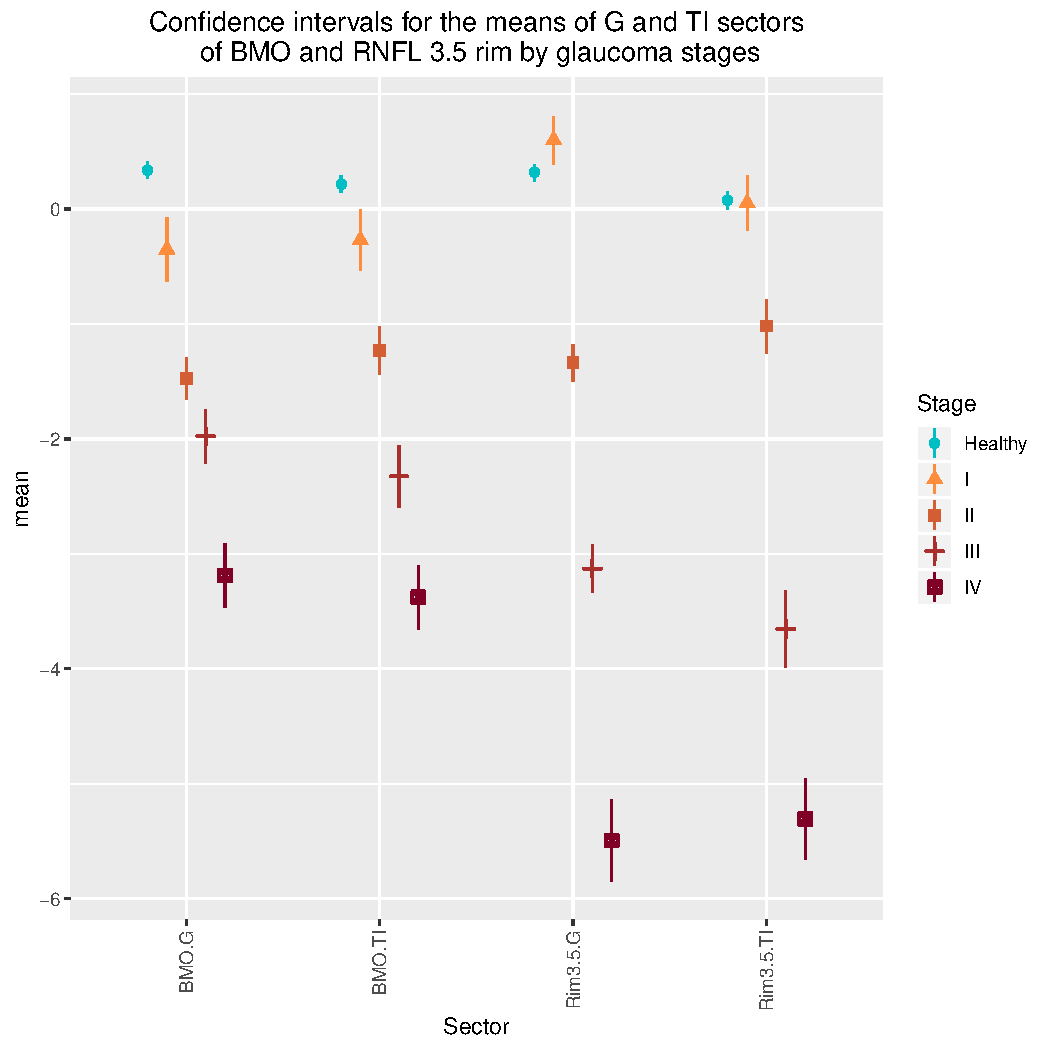
\includegraphics[width=0.5\linewidth]{img/confidence-intervals-bmo-35-G-TI-stages.pdf}
\caption{Distribution of the first principal component of the BMO-MRW and RNFL rim variables by glaucoma stages and healthy eyes.}
\label{fig:confidence-intervals}
\end{figure}

Finally, to render this staging system operational, we developed an online application (app) that implements this classification model. Figure~\ref{fig:glaucoma-app} shows a screenshot of the app. In this simple app, the user must provide a subject’s age and the BMO-MRW area, which are required for standardization, and the measurements for sectors G and TI of the BMO-MRW and RNFL 3.5 rim, and the app returns the glaucoma stage prediction for the eye and the probability for each stage. The app also plots the position of the eye on the two first principal components’ planes relative to the clusters of the different stages. The app is currently available at \url{https://asalberapps.shinyapps.io/Glaucoma-Staging-System/}.

\begin{figure}[ht]
\centering
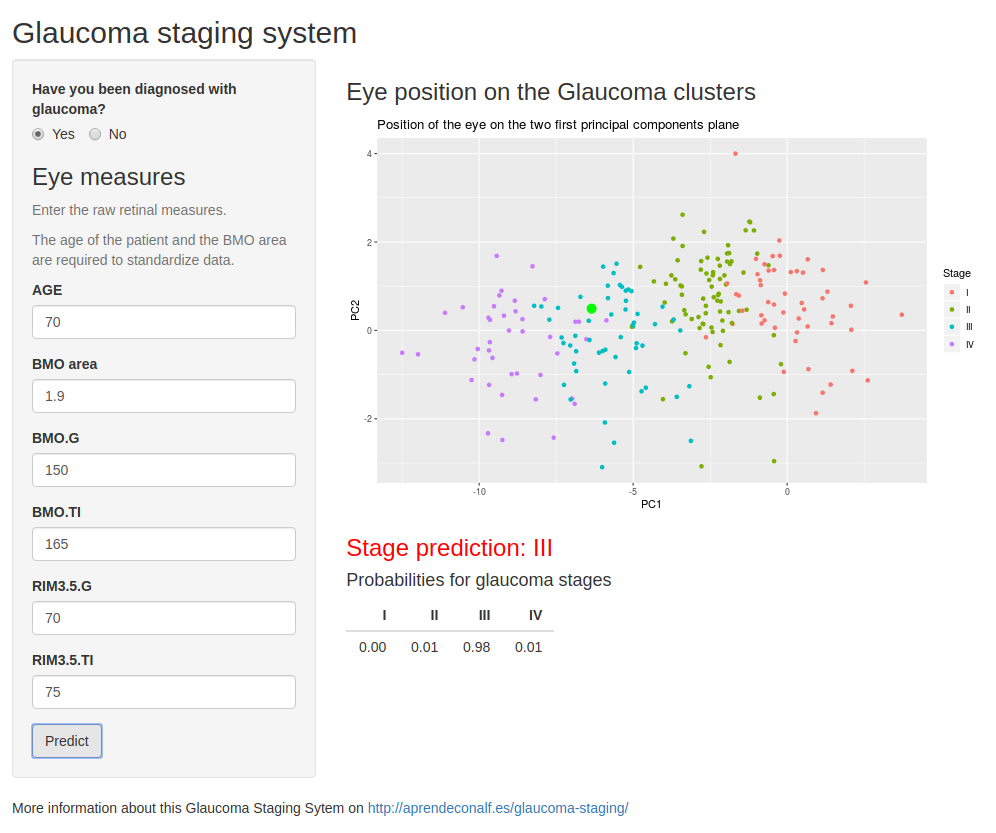
\includegraphics[width=0.8\linewidth]{img/glaucoma-staging-app.png}
\caption{Classification of one eye using the glaucoma-staging app.}
\label{fig:glaucoma-app}
\end{figure}

\section*{Discussion}

Even after OCT emergence, one constant in the attempt to classify POAG was the VF. Our study does not consider the VF to be a classification element due to its subjective nature because of arbitrary limits of exclusion according to fixed losses, false-positives, cognitive impairment, and difficult collaborations. VF-based classifications have been proposed, and multiple reviews of these classifications have been published \cite{germano:2017:evaluation, hirasawa:2013:} \textcolor{red}{(Hirasawa,Shoji, Morita,Shimizu, 2013b; Ng et al., 2012)}. A summary of all of these reviews may yield a strong conclusion. The presence of glaucomatous optic neuropathy increases with the severity of staging for all systems. However, different systems led to different stages of severity \textcolor{red}{(Ng  et al., 2012)}.

Other proposals for the diagnosis and classification of POAG have recently been presented based on OCT angiography\cite{mansoori:2018:optical,miguel:2019:diagnostic,rabiolo:2018:comparison,hollo:2018:optical,saba:2018:fundus}. All of these proposals, whether based on retrospective reviews of articles\cite{saba:2018:fundus} or personal work, reveal the potential of this technique, but they also introduce uncertainty due to inconsistent criteria in terms of the diagnosis of glaucoma and especially glaucoma’s classification. We think that imaging examinations introduce elements such as anatomical anomalies, exudates, haemorrhage, and the distorting effect of the vessels on the nasal side of the papilla, which can lead to misinterpretation. Therefore, we considered the actual anatomical shape of the papilla limits, the BMO-MRW \textcolor{red}{(Chauhan et al. falta año)}, and the normalized values of the BMO-MRW and RNFL to be objective, accessible, and reproducible variables to propose a clinical-evolutionary classification system of glaucoma.

The diagnostic accuracy of sectoral or global analyses of RNFL and/or BMO-MRW has also been performed in glaucoma. Danthurebandara et al. \cite{danthurebandara:2016:diagnostic} reported that with a normative limit of 1\%, sectoral analysis of the BMO-MRW-HRW showed a sensitivity of 87\% and a specificity of 92\%, while global analysis yielded the same specificity (92\%) but a sensitivity of 88\%. With higher normative limits, the values decreased. The authors concluded that both parameters had similar diagnostic accuracies.

Fan et al. \cite{fan:2017:enhanced} sought to improve the diagnostic capacity of the three-dimensional (3D) neuroretinal edge parameters with the nerve edge thickness (RNFL) and the two-dimensional RNFL using SD-OCT. Among the three parameters of the 3D edges (\textcolor{red}{MDB}, BMO-MRW), no significant differences were found in the diagnostic capacity (false detection rate > 0.05 with a specificity of 95\%).

Authors such as Zheng et al. \cite{zheng:2019:diagnostic} have also worked with the inferotemporal and superotemporal sectors of the RNFL to improve the sensitivity and specificity with respect to the same sectors of the BMO-MRW with POAG campimetry and percentiles < 5. Abnormal superotemporal and/or inferotemporal RNFL thicknesses achieved a higher sensitivity than abnormal superotemporal and/or inferotemporal BMO-MRWs in the detection of mild glaucoma. The mean DM of the VF: -3.32 $\pm$ 1.59 dB (97.9\% and 88.4\%, respectively, p = 0.006) and the mean DM of the VF -9.36 $\pm$ 8.31 dB (98.4\% and 93.6\%, respectively, p = 0.006), with the same specificity (96.1\%). We think that below the 5th percentile, the best definitions are of little significance when more specific sectors such as G and IT are not studied.

In our study, we relied on artificial intelligence (AI) for having potential for the detection, diagnosis, and classification of glaucoma, both through the automated processing of large data sets and through the early detection of new patterns of diseases \cite{zheng:2019:artificial}, and we considered the parameter BMO-MRW to be important when defining the stages of the disease, as shown in Table~\ref{tab:model-comparison}.\cite{chauhan:2013:enhanced} Valuing the diagnostic capacities of the parameters RNFL thickness, BMO-MRW-HRW and BMO-MRW showed that the BMO-MRW with a specificity of 95\% had a higher sensitivity than the rest of the parameters studied, with sensitivities of 70\%, 51\% and 81\%, respectively.

Brusini \cite{brusini:2018:glaucoma} proposed a classification with similarities to our classification but also with definitive differences. Brusini’s classification uses the upper and lower RNFL thickness values plotted in a Cartesian plane to classify glaucoma OCT results. RNFL defects are classified into six stages of increasing severity and three classes of defect location (upper, lower, or diffuse defects). The diagram was created based on 302 tests of OCT in 94 healthy controls and 284 patients affected by perimetric POAG.

Our study was proposed in a more practical and simpler manner, with incorporation of a patient with ocular hypertension without campimetric damage and a patient with POAG with campimetric damage. We note some substantial differences. First, we includehttps://www.overleaf.com/project/5da5abb74dc7c00001698670d more variables that suffer the effect of IOP; in the BMO-MRW and RNFL sectors (28 variables in total), Brusini only consider the RNFL. We believe in the importance of the BMO-MRW as we have historically focused on different means to verify the behaviour of vessel displacement and evaluate the cribriform plate in the papillary excavation \cite{reis:2012:influence}. We corroborate the importance of the BMO-MRW in determining the severity of glaucoma because of its variables, particularly the BMO-MRW.G, which is included in the classification model presented in table~\ref{tab:model-comparison}, where sector G of the BMO-MRW and the 3.5 rim yield a similar sensitivity and specificity when considering the 28 sectors.

Brusini considered the mean thicknesses of the upper and lower quadrants of the RNFL, ignoring other variables because they are not reliable in the determination of structural damage, although no justification for these variables’ exclusion is provided. We propose consideration of all sectors of the RNFL and BMO-MRW (NI, N, NS, TS, T, and TI) in addition to a global measure (G) that averages 728 points in each rim, and we select those sectors with greater discriminatory power in the final classification model (sectors that simplify the equation of the first principal component). 

Brusini proposes six groups of increasing severity for the classification of POAG in an arbitrary manner that does not obey objective or statistical criteria.  In our work, four classes were established because this number is optimal in terms of reducing intra-group variability according to the k-means algorithm. A greater number of classes does not substantially reduce the total intra-group variability, as shown in Figure 5.

The groups that Brusini established are separated in the Cartesian plane in the direction of the two variables considered by taking intervals of equal length in the x- and y-axes, but these axes do not correspond to the directions of the maximum variability of the data, which would be the directions of the principal components.  

Our groups are very well separated in the direction of the first principal component, as shown in Figure 6. When using the k-means algorithm, the resulting groups do not have the same size but emerge more naturally by agglutination around the means of each group.
With respect to validation of the classification model, Brusini’s only studies the sensitivity (0.85-0.95) and specificity (0.92-0.98) for the distinction between patients with campimetric damage and healthy patients and not for the distinction between different stages. Our results, which include ocular hypertensive patients (without campimetric damage), validate the system with a mean sensitivity and specificity of 0.94 for group I, 0.94 for group II, 0.96 for group III and 0.98 for group IV. Groups I and II show lower values for being in the area of ocular hypertension, which could be considered a preclinical and precampimetric stage, in which the variables studied are close to normal values (Table 3).

When we introduce healthy patients, the results may lose statistical power due to their values, but they can discriminate between healthy and glaucomatous eyes with average values of 0.79. When we classify an individual without knowing whether he or she has glaucoma, we classify him or her into stages with mean sensitivity and specificity values of 0.72 for stage I and 0.90 and 0.95 for stages III and IV, respectively.

Our classification algorithm not only demonstrates its functionality within a group of known glaucomatous patients but can also be useful for the diagnosis of POAG in general population surveys because although its performance in early stages of glaucoma (I and II) shows low sensitivity and specificity, significant values are reached at more advanced stages (III and IV), enabling diagnosis with a mean global precision of 0.88. 
Considering the robustness of our study due to verification and evaluation of 1001 patients, 235 of whom had glaucoma at various stages of evolution, we can accept that only a single tomographic scan was considered for the study (the last scan performed). This test was considered the examination that would define the current state of the process.

In conclusion, we consider this new classification important for an individual understanding of each patient with POAG or even other types of glaucoma. We provide a common language to refer to the clinical-evolutionary development of POAG and to facilitate the decision regarding treatment aggressiveness depending on the stage of glaucoma or the evolutionary speed within the stages, especially . in the intermediate and advanced stages.

\section*{Methods}

\subsection*{Study design and patient selection}

We plan an analytical, observational, cross-sectional and comparative study of patients with ocular hypertension and patients with POAG who were consecutively treated at Policlínica Baza and Clínica Vistacamacho (Almería) between May 2016 and June 2018. The patients were informed about the nature of the study, agreed to participate anonymously, and provided informed consent under the current data protection law. The study adhered to the conditions of the Declaration of Helsinki (sixth revision, 2008) and was approved by the ethics committee of the participating centres.

A complete ophthalmological examination was performed during the inclusion session, which included best-corrected visual acuity , cycloplegic refractions (Tropicamide 1\%), visual acuity with best correction, measurement of central corneal thickness by ultrasound pachymetry, slit-lamp examination and gonioscopy, and a retinal and optic nerve funduscopy with 78-dioptric hand lens.

\subsection*{Inclusion criteria}

All patients had to meet the following criteria to be selected: (A) A cognitive ability to accept and understand the proposed procedures; (B) a clinical record of intraocular pressure (IOP)> 23 indicative of ocular hypertension (OH) in the absence of campimetric damage, a normal optic disc (NOP) and all sector values assessed by SD-OCT within normal percentiles; (C) POAG with historical clinical records of a IOP> 23 at least once; such patients should have received anti-hypertensive treatment and/or surgery six months earlier. These patients had to have a minimum of two clinical records, a VF < 20\% considering false-negative and false-positive responses, and < 20\% fixation losses as well as glaucomatous defects according to the Hodapp classification. The VF tests were performed using the standard Swedish interactive threshold algorithm (SITA) target and VF target strategy with a Humphrey II field analyser (software version 4, program 24-2, Goldmann objective size III, a stimulus duration of 200 ms, model HFA 740, Humphrey Instruments, Inc., Dublin, CA, USA); (D) Caucasian race; (E) the absence of diseases in the retina or optic nerve; (F) open-angle verification by gonioscopy as well as the absence of signs of pseudoexfoliation and pigmentary glaucoma.

\subsection*{Criteria for exclusion}

Ocular hypertensive patients or POAG patients were excluded from the study if they (A) did not agree to participate or did not meet the inclusion criteria, (B) had a direct family history of cognitive neurodegenerative diseases or exhibited suspicious signs, (C) had diseases in the retina and optic nerve before or at the time of inclusion, (D) had undergone intraocular surgeries in the previous 6 months, except for successful cataract removal or surgeries related to POAG, (E) exhibited non-transparent media at any level, (F) had severe systemic diseases, (G) had refractive errors above the spherical equivalent of three dioptres, (H) had SD-OCT tests with signal strengths lower than 20, or (I) were initially considered hypertensive and did not have elevated IOP values after three months of anti-hypertensive treatment and discontinuation of such treatment.

SD-OCT was performed on all patients on one side to avoid problems related to a correlation between the eyes of the same patient. OCT was performed with the Heidelberg Spectralis device (Heidelberg Engineering, GmbH. Germany, Software Heidelberg Eye Explorer ver. 6.7c).

The glaucoma program provided by the manufacturer was used, which has a patented anatomical positioning system (APS) with a series of patterns for scanning of the optic nerve head, the RNFL, and the macular ganglion cell layer. The program compares the eyes of patients with normalized baseline values for normal eyes.

No segmentations were performed manually.

The absolute values of healthy, glaucomatous and hypertensive eyes prior to normalization indicated by Heidelberg Engineering and obtained from the seven sectors of the BMO-MRW and the three peripapillary rims (G-TS-T-TI-NS-N-NI) were exported to a Microsoft Excel (version 2016; Microsoft Corporation, Redmon, WA, USA) table. These absolute values were adjusted for age and the area of the papillary cup and normalized following the indications of Heidelberg Engineering using the following formula provided by Heidelberg Engineering:

\[
z_i=\frac{x_i-\bar x-b_{xe}(e_i-\bar e)-b_{xa}(a_i-\bar a)}{s_x}
\]

where:
\begin{itemize}
\setlength\itemsep{0pt}
\item[] $x_i$ is the value of individual $i$ in variable $x$.
\item[] $\bar x$ is the mean of variable $x$.
\item[] $s_x$ is the standard deviation of variable $x$.
\item[] $e_i$ is the age of individual $i$.
\item[] $\bar e$ is the mean age of healthy individuals at baseline.
\item[] $b_{xe}$ is the slope of the regression line of variable $x$ on age.
\item[] $a_i$ is the area of the BMO-MRW of individual $i$.
\item[] $\bar a$ is the mean area of the BMO-MRW of healthy individuals at baseline.
\item[] $b_{xa}$ is the slope of the regression line of variable $x$ over the area of the BMO-MRW.
\item[] $z_i$ is the standardized value of individual $i$ in variable $x$.
\end{itemize}

\subsection*{Statistical analysis}

Data processing and analysis were performed with the programs R (version 3.5), RKWard (version 7.0) and rk.Teaching (package) (version 1.3)\cite{sanchez:2015:bringing}. 

The normality of RNFL variables was proven with the Kolmogorov-Smirnov test, and the homogeneity of variances was tested with Box’s M test using an $\alpha$ level of $0.05$.

To cluster the eyes into stages of glaucoma, we used the k-means method (Trevor, Robert, 2009). For the classification, we used LDA (Trevor, Robert, 2009). The classification power with this technique was evaluated by cross-validation. 

The data and all the results of this study are publicly available at \url{https://github.com/asalber/glaucoma-staging} and \url{http://aprendeconalf.es/glaucoma-staging/}.

\bibliography{bibliography}

\section*{Author contributions statement}

Design of the experiment (J.G. and A.S.);  Data collection (A.P.); Data analysis (A.S.); Interpretation of results (J.G., A.S. and A.P.); Writing the article (A.P. and A.S.); Criticla review of the article (J.G.).

\section*{Additional information}
\textbf{Supplementary information} accompanies this paper at \url{http://aprendeconalf.es/glaucoma-staging/}.

\medskip

\noindent\textbf{Competing interests}: The author(s) declare no competing interests.

\end{document}